% Created 2018-05-20 Dom 16:33
\documentclass[11pt]{article}
\usepackage[utf8]{inputenc}
\usepackage[T1]{fontenc}
\usepackage{fixltx2e}
\usepackage{graphicx}
\usepackage{longtable}
\usepackage{float}
\usepackage{wrapfig}
\usepackage{rotating}
\usepackage[normalem]{ulem}
\usepackage{amsmath}
\usepackage{textcomp}
\usepackage{marvosym}
\usepackage{wasysym}
\usepackage{amssymb}
\usepackage{hyperref}
\tolerance=1000
\usepackage[margin=2cm]{geometry}
\author{Cecília Carneiro e Silva}
\date{23/05/2018}
\title{RNA-TRAB11}
\hypersetup{
  pdfkeywords={},
  pdfsubject={},
  pdfcreator={Emacs 25.3.1 (Org mode 8.2.10)}}
\begin{document}

\maketitle

\section{Redes concorrentes}
\label{sec-1}

O objetivo deste exemplo é construir uma \textbf{Rede Neural Competitiva} para formar uma \textbf{Look-up table} para a função: y = 1/x. A quantidade de cluster será variada dos exemplos. A entrada é uma lista, em ordem randômica, de pares '(x y) que obedencem a função acima. 

\begin{verbatim}
- Entrada: (range 1 10 0.001), 9001 entradas
'((1 1.0) ... (9.999999999999897 0.10000000000000103))
\end{verbatim}

\subsection{Considerações}
\label{sec-1-1}

\begin{itemize}
\item Pesos iniciais gerados aleatoriamente.
\item Atualização dos pesos:
\end{itemize}

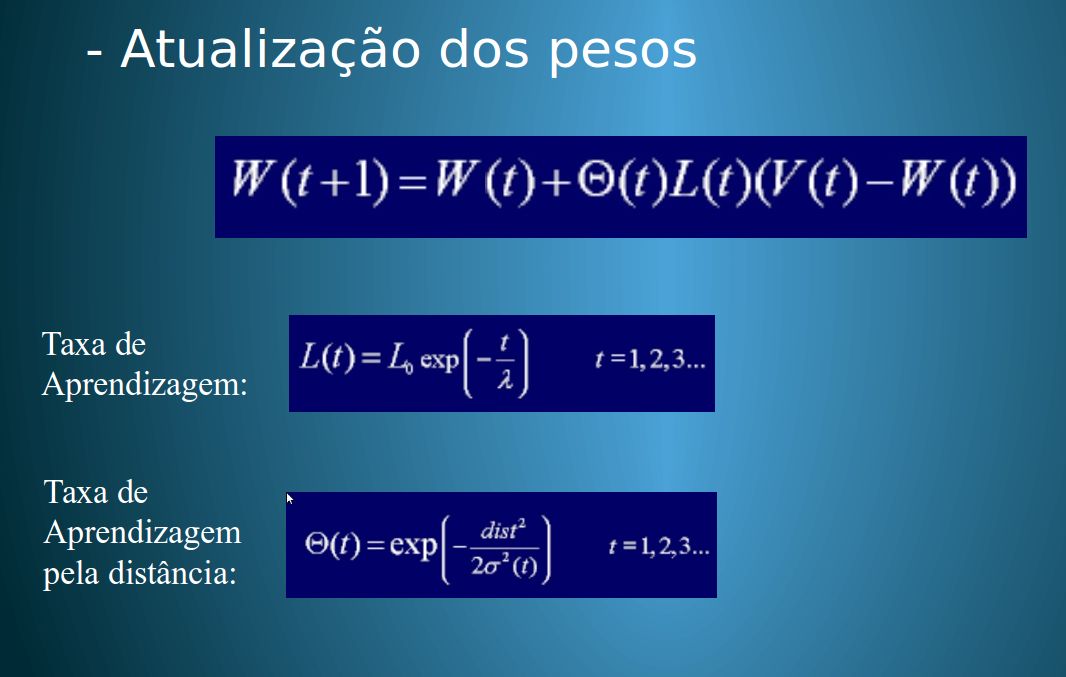
\includegraphics[width=.9\linewidth]{images/w-update.png}

\begin{itemize}
\item Parada: quando $\Delta$ w for melhor do que a precisão (1e-10).
\end{itemize}

\subsubsection{Testes}
\label{sec-1-1-1}

\begin{verbatim}
;;(define 1divx (shuffle (1divx_fun 10)))
> (network_som input_list n_output_x radius_max n_iterations_max [n_output_y 1])
\end{verbatim}

\subsection{Teste 1}
\label{sec-1-2}
\begin{itemize}
\item Cluster: 10
\item Raio máximo: 5
\item Iterações-cálculos: 1000
\end{itemize}

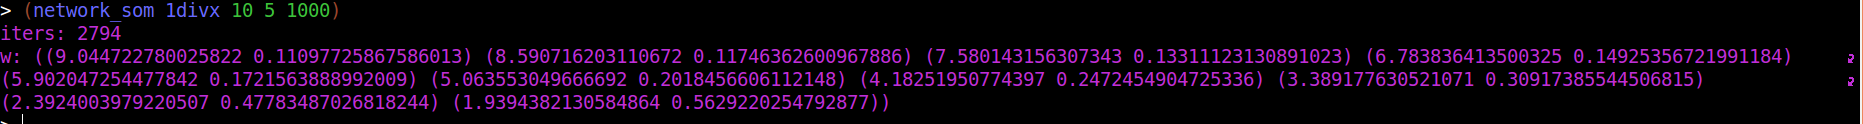
\includegraphics[width=.9\linewidth]{images/t1-results.png}

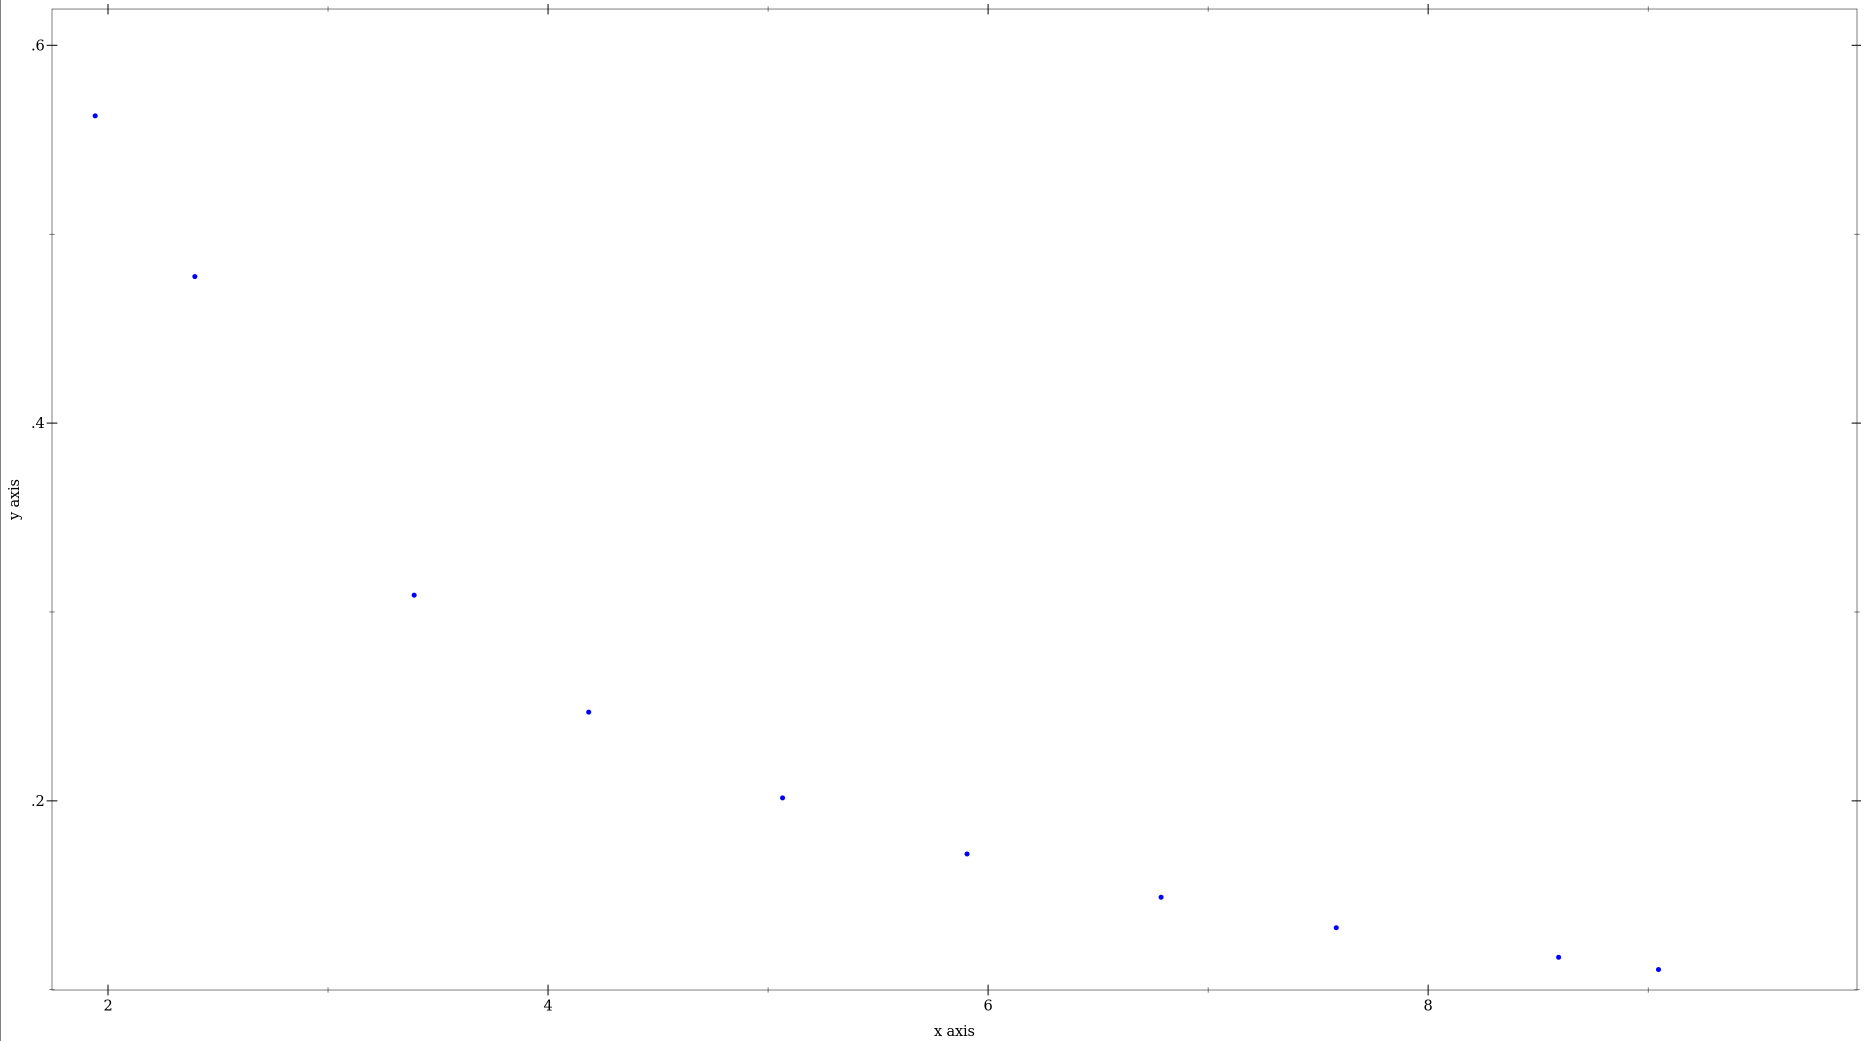
\includegraphics[width=.9\linewidth]{images/t1-plot.png}

\subsection{Teste 2}
\label{sec-1-3}
\begin{itemize}
\item Cluster: 12
\item Raio máximo: 5
\item Iterações-cálculos: 1000
\end{itemize}

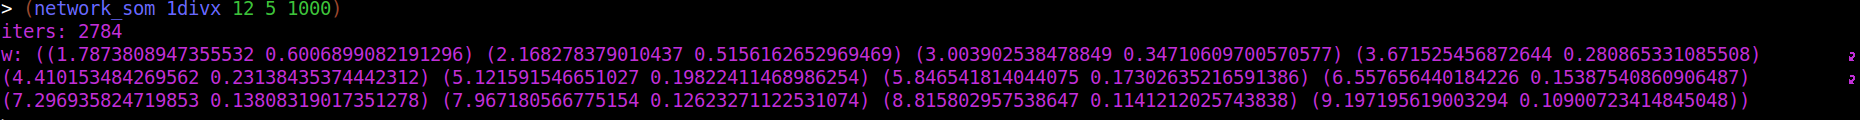
\includegraphics[width=.9\linewidth]{images/t2-results.png}

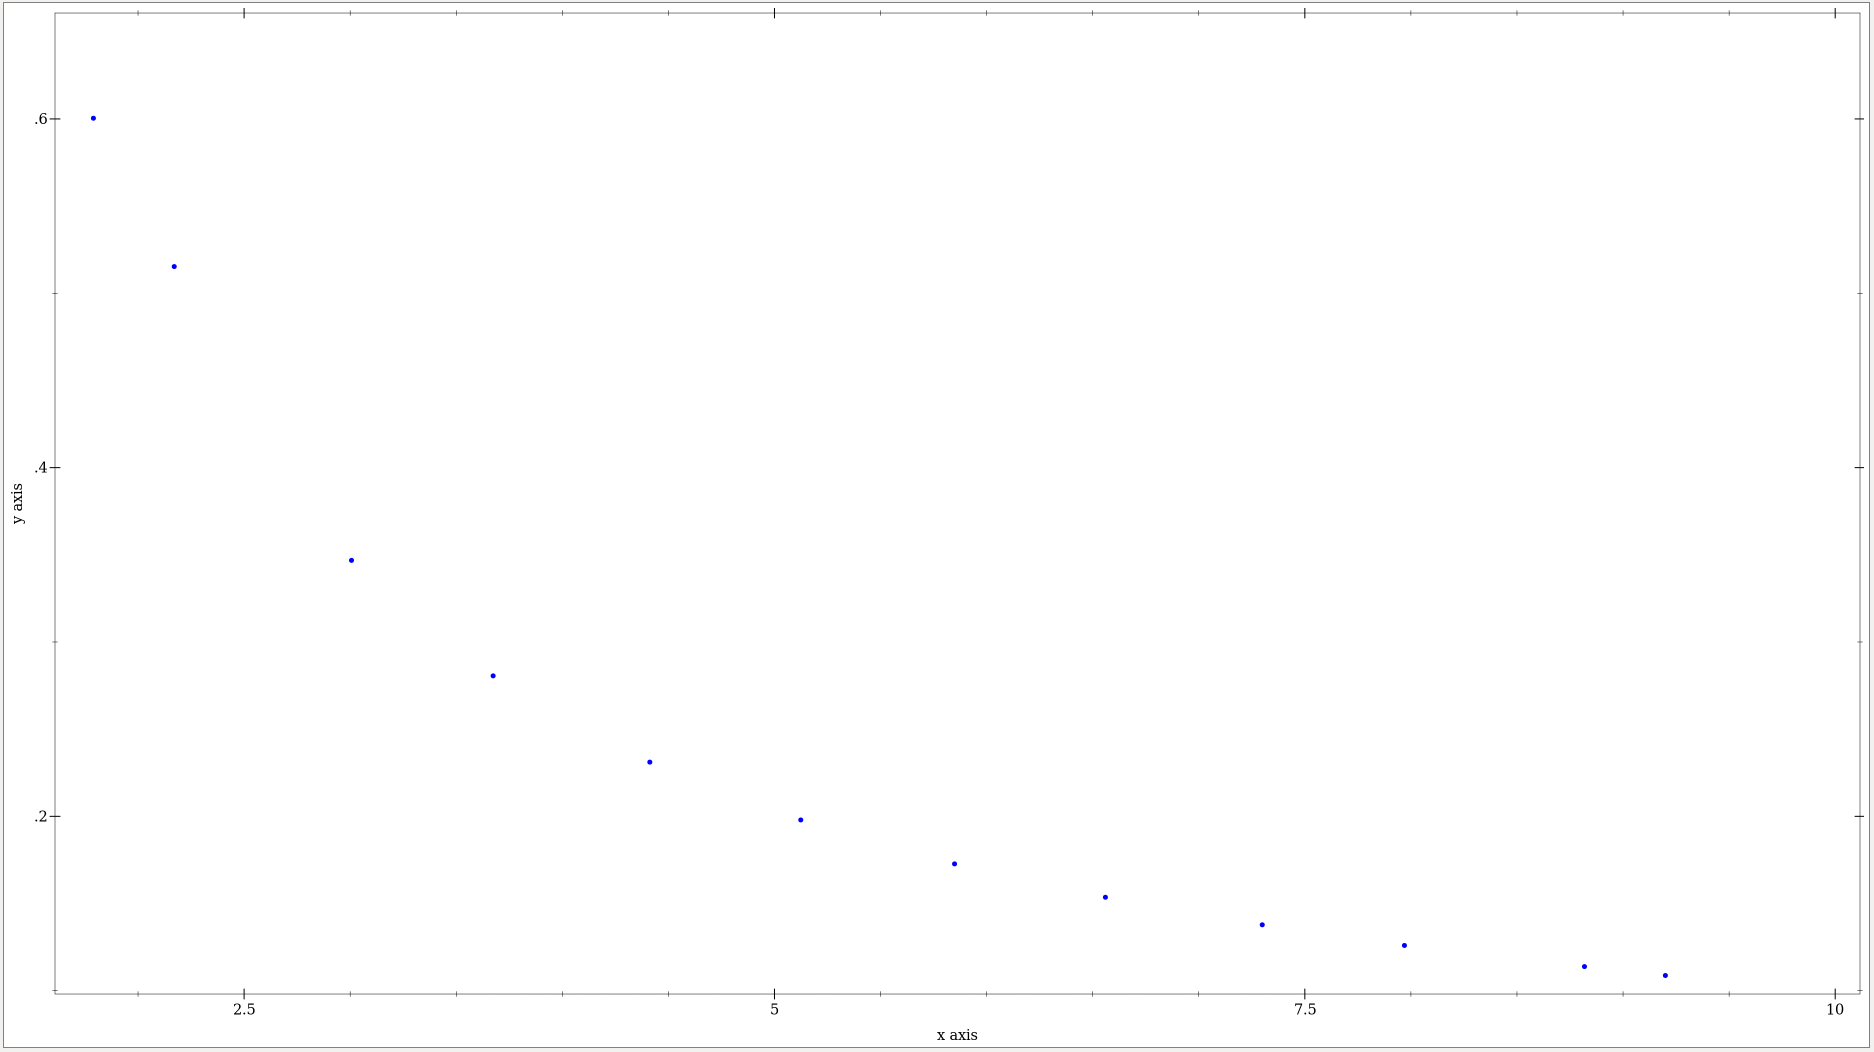
\includegraphics[width=.9\linewidth]{images/t2-plot.png}
% Emacs 25.3.1 (Org mode 8.2.10)
\end{document}
